\chapter{Central Spin Model}

\begin{wrapfigure}{r}{0.4\textwidth}
    \centering
    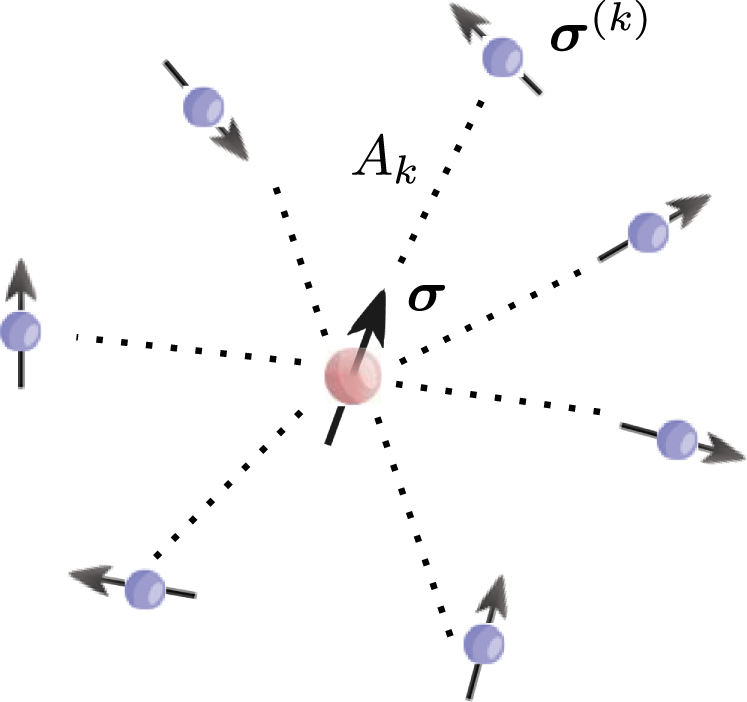
\includegraphics[width = 0.35\textwidth]{Abbildungen/CSM_Schema.jpg}
    \caption{Schematischer Aufbau des Central-Spin-Modells mit dem Elektronenspins (Rot) und den in direkter Umgebung liegenden 
    Kernspins (Blau) und einer Kopplungskonstante $A_k$}
    \label{fig:CSM}
\end{wrapfigure}
%CSM: https://iopscience.iop.org/article/10.1088/1367-2630/16/6/065023
Im folgenden wir das \textbf{Central Spin Model} zur Beschreibung der Spindynamik des Quantenpunktes verwendet. Dabei werden 
zu dem vorherigen Hamiltonian, die legiglich die Interaktionen des Elektrones mit mit einem externem Magnetfeld $\vec{B}$ berücksichtigt, 
fließen die Interaktionen der umliegenden Kernspins $\hat{\vec{I}}_k$ mit ein, d.h. die Wechselwirkung der Kernspins mit dem externen 
Magnetfeld und dem Elektronen-Spin über eine Heisenbergkopplung mit der Kopplungskonstante $A_k$. Die Wechselwirkungen, der einzelnen Kernspins 
untereinander wird vernachlässigt.

\begin{align}
    \overline{\hat{H}}_{CSM} &= \mu_B\thinspace g_e \vec{B}\hat{\vec{S}} +  \sum_{k=1}^{N}\mu_k\thinspace g_k\vec{B}\hat{\vec{I}}_k + \sum_{k=1}^{N} A_k \hat{\vec{S}}\hat{\vec{I}}_k
\end{align}
Dabei entspricht anders als beim freien Elektron der g-Faktor eines Elektron im Quantenpunkt nicht mehr 2, sondern ca. 0,555. %[A. Greilich, A. Shabaev, D. R. Yakovlev, Al. L. Efros, I. A. Yugova, D. Reuter,
%A. D. Wieck, and M. Bayer. Nuclei-induced frequency focusing of electron spin
%coherence. Science, 317:1896, 2007.]
Das Kernmagneton $\mu_k= 5,05 \cdot 10^{27} \frac{J}{T}$ ist etwa 1800 Mal kleiner als das Bohrsche Magneton.
Die g-Faktoren $g_k$ können für alle Kernspins der Einfachheit Halber als gleich angenommen werden. Zudem lässt sich eine charakterische Zeit
definieren:
\begin{align}
    T^* &= \frac{1}{\sqrt{\sum_k A_k^2\langle \hat{I}_k^2 \rangle}}
\end{align}

Nun kann der dimensionslose Hamiltonian $\hat{H}_{CSM} = T^*\thinspace\overline{\hat{H}}_{CSM}$ hingeschrieben werden:

\begin{align}
    \hat{H}_{CSM} &= \vec{b}\hat{\vec{S}} +  \sum_{k=1}^{N}z_k\vec{b}\hat{\vec{I}}_k + \sum_{k=1}^{N} \alpha_k \hat{\vec{S}}\hat{\vec{I}}_k
\end{align}
% \langle\Psi(t) \mid \dot{\Psi}(t)\rangle

mit $\vec{b}=T^*\mu_B\thinspace g_e \vec{B}$ , $z_k=T^*\frac{\mu_I g_k}{\mu_B g_e}$ und $\alpha_k = T^* A_k$.

\noindent Durch die Hinzunahme nur eines zusätzlich Kernspinors $\hat{\vec{I}}$ erhalten wir den einfachsten Fall des Central 
Spin Models, der Hamiltonian vereinfacht sich somit zu:

\begin{align}
    \hat{H} &= \underbrace{ \vec{b}\hat{\vec{S}}}_{\hat{H}_1} + \underbrace{z \vec{b}\hat{\vec{I}}}_{\hat{H}_2} + 
    \underbrace{\alpha \hat{\vec{S}}\hat{\vec{I}}}_{\hat{H}_3}\\
\end{align}

 mit der charakteristischen Zeit:

 \begin{align}
    T^* &= \sqrt{\frac{4}{3}}\frac{1}{A}
 \end{align}



%%%%%%% Klassischer Ansatz





\section{klassischer Ansatz}
\noindent Im ersten Schritt wird der klassische nicht-normierte Produktansatz $\ket{\Psi} = \ket{\Psi(\mu_1, \mu_2)}$: 
\begin{align}
    \ket{\Psi} &= e^{\mu_1 S_{1}^{-}}e^{\mu_2 S_{2}^{-}}\ket{\uparrow,\uparrow}\\
                &= \ket{\uparrow \uparrow} +\mu_1\ket{\downarrow \uparrow} + \mu_2\ket{\uparrow \downarrow} + \mu_1\mu_2\ket{\downarrow\downarrow}\\
                &= \underbrace{\left(\ket{\uparrow}_1 + \mu_1\ket{\downarrow}_1\right)}_{\ket{\Psi_1}}\underbrace{\left(\ket{\uparrow}_2 + \mu_2\ket{\downarrow}_2\right)}_{\ket{\Psi_2}}  \\
\end{align}

Mit diesem Produktansatz ergeben sich die Spin-Erwartungswerte:
\begin{align}
    \frac{\bra{\Psi}\hat{S_x}\ket{\Psi}}{\N} &= \frac{1}{2}\frac{\muk_1 + \mu_1}{1+\mu_1\muk_1} = \frac{Re[\mu_1]}{1 + \mu_1\muk_1} \\
    \frac{\bra{\Psi}\hat{S_y}\ket{\Psi}}{\N} &= \frac{i}{2}\frac{\muk_1 - \mu_1}{1+\mu_1\muk_1} = \frac{Im[\mu_1]}{1 + \mu_1\muk_1} \\
    \frac{\bra{\Psi}\hat{S_z}\ket{\Psi}}{\N} &= \frac{1}{2}\frac{1 - \mu_1\muk_1}{1 + \mu_1\muk_1}  
\end{align}
und 
\begin{align}
    \frac{\bra{\Psi}\hat{I_x}\ket{\Psi}}{\N} &= \frac{1}{2}\frac{\muk_2 + \mu_2}{1+\mu_2\muk_2} = \frac{Re[\mu_2]}{1 + \mu_2\muk_2} \\
    \frac{\bra{\Psi}\hat{I_y}\ket{\Psi}}{\N} &= \frac{i}{2}\frac{\muk_2 - \mu_2}{1+\mu_2\muk_2} = \frac{Im[\mu_2]}{1 + \mu_2\muk_2} \\
    \frac{\bra{\Psi}\hat{I_z}\ket{\Psi}}{\N} &= \frac{1}{2}\frac{1 - \mu_2\muk_2}{1 + \mu_2\muk_2}
\end{align}



Damit ergibt sich für den modifizierten Hamiltonian: 

\begin{align}
    \mathcal{H} &= \frac{\bra{\Psi}\hat{H}_1\ket{\Psi}+ \bra{\Psi}\hat{H}_2\ket{\Psi} +\bra{\Psi}\hat{H}_3\ket{\Psi}}{\N}\\
\end{align}

Mit

\begin{align}
   \bra{\Psi}\hat{H_1}\ket{\Psi} &= \frac{1}{2}(1+\mu_2\muk_2)\left(b_x(1-\mu_1^2) + ib_y(1+\mu_1^2) - 2\mu_1 b_z\right)\\
   \bra{\Psi}\hat{H_2}\ket{\Psi} &= \frac{z}{2}(1+\mu_1\muk_1)\left(b_x(1-\mu_2^2) + ib_y(1+\mu_2^2) - 2\mu_2 b_z\right)\\
   \bra{\Psi}\hat{H}_3\ket{\Psi} &= \frac{\alpha}{4}\left[( \mu_1 + \muk_1)( \mu_2 + \muk_2) - (\mu_1-\muk_1)(\mu_2 - \muk_2) + (1-\mu_1\muk_1)(1-\mu_2\muk_2)\right]
\end{align}  


Und wir erhalten die partiellen Ableitungen:
\begin{align}
    \partial_{\muk_1}\mathcal{H} &= \underbrace{\frac{1}{2(1+\mu_1\muk_1)^2}[b_x(1-\mu_1^2) + ib_y(1+\mu_1^2) - b_z\mu_1]}_{= \partial_{\muk_1} \frac{\bra{\Psi}\hat{H}_1 + \hat{H}_2\ket{\Psi}}{\N}} \\
    &+ \underbrace{\frac{\alpha}{2}\frac{(\mu_2 -\mu_1)(1+\mu_1\muk_2)}{(1+\mu_1\muk_1)^2(1+\mu_2\muk_2)}}_{= \partial_{\muk_1} \frac{\bra{\Psi}\hat{H}_3\ket{\Psi}}{\N}}\\
    \partial_{\muk_2}\mathcal{H} &= \underbrace{\frac{z}{2(1+\mu_2\muk_2)^2}[B_x(1-\mu_2^2) + iB_y(1+\mu_2^2) - B_z\mu_2]}_{= \partial_{\muk_2} \frac{\bra{\Psi}\hat{H}_1 + \hat{H}_2\ket{\Psi}}{\N}} \\
    &+ \underbrace{\frac{\alpha}{2}\frac{(\mu_1 -\mu_2)(1+\mu_2\muk_1)}{(1+\mu_1\muk_1)(1+\mu_2\muk_2)^2}}_{= \partial_{\muk_2} \frac{\bra{\Psi}\hat{H}_3\ket{\Psi}}{\N}}
\end{align}

Um nun die DGL aufzustellen, fehlt nur noch die Berechnung der modifizierten Gram-Matrix, die diesmal zweidimensional ist. 
Wir erhalten nach einer längeren Rechnung:

\begin{align}
    G &=
    \begin{pmatrix}
        (1+\mu_1\muk_1)^2 & 0 \\
        0 &(1+\mu_2\muk_2)^2
    \end{pmatrix} \\
    G^{-1} &=
    \begin{pmatrix}
        \frac{1}{(1+\mu_1\muk_1)^2} & 0 \\
        0 &\frac{1}{(1+\mu_2\muk_2)^2}
    \end{pmatrix}
\end{align}

\noindent Nun können die Bewegungsgleichungen aufgestellt werden:
\begin{align}
    i\dot{\mu_1} &= \sum_{j}\left(G_{1j}\right)^{-1}\thinspace \partial_{\overline{\mu_j}}\mathcal{H}  \\
    &=\underbrace{\frac{1}{2}b_x(1-\mu_1^2) + \frac{i}{2}b_y(1+\mu_1^2) -\mu_1 b_z}_{\text{Ein-Spin-Präzession im } \vec{B}} +\underbrace{\frac{\alpha}{2} \frac{(\mu_2-\mu_1)(1+\mu_1\muk_2)}{1+\mu_2\muk_2}}_{\text{Ein-Spin-Präzession um } \frac{\bra{\Psi}\hat{\vec{I}}\ket{\Psi}}{\N}  }    
\end{align}
und analoger Weise 
\begin{align}
    i\dot{\mu_2} &= \underbrace{\frac{z}{2}b_x(1-\mu_2^2) + \frac{iz}{2}b_y(1+\mu_2^2) -\mu_2 z b_z}_{\text{Ein-Spin-Präzession im } \vec{B}} +\underbrace{\frac{\alpha}{2} \frac{(\mu_1-\mu_2)(1+\mu_2\muk_1)}{1+\mu_1\muk_1}}_{\text{Ein-Spin-Präzession um } \frac{\bra{\Psi}\hat{\vec{S}}\ket{\Psi}}{\N}  }
\end{align}

\noindent Aufgrund der Linearität der DGL ist die Lösung der ersten DGL aus dem Ein-Spin-Fall zu entlesen. Nun fehlt es noch zu beweisen, 
dass der letztere Summand die Präzession um den Spin-Erwartungswert des jeweilig anderen Spins beschreibt. Wenn dieser Ansatz angenommen wird,
kann durch auflösen die Gleichheit gezeigt werden:  

\begin{align}
     \frac{\alpha}{2}\left[\underbrace{\frac{1}{2}\frac{\mu_2 + \muk_2}{1+\mu_2\muk_2}}_{\frac{\bra{\Psi}\hat{I}_x\ket{\Psi}}{\N}}(1-\mu_1^2) 
     + i \underbrace{\frac{i}{2}\frac{\muk_2 -\mu_2}{1+\mu_2\muk_2}}_{\frac{\bra{\Psi}\hat{I}_y\ket{\Psi}}{\N}}(1+\mu_1^2) 
     - 2\mu_1\underbrace{\frac{1}{2}\frac{1-\mu_2\muk_2}{1+\mu_2\muk_2}}_{\frac{\bra{\Psi}\hat{I}_z\ket{\Psi}}{\N}} \right]
     &= \frac{\alpha}{2} \frac{(\mu_2-\mu_1)(1+\mu_1\muk_2)}{1+\mu_2\muk_2}
\end{align}
Hier lässt sich erkennen, dass die $\frac{\bra{\Psi}\hat{I_i}\ket{\Psi}}{\N}$ die Rolle des Magnetfeldes $\vec{B}$ im Ein-Spin-Lösung 
übernehmen. Wir erhalten dann aus Symmetriegründen:

\begin{align}
    \frac{d}{dt}\left[\frac{\bra{\Psi}\hat{\vec{S}}\ket{\Psi}}{\N}\right] &= \left(\vec{b} + \alpha \frac{\bra{\Psi}\hat{\vec{I}}\ket{\Psi}}{\N}\right)\cross\frac{\bra{\Psi}\hat{\vec{S}}\ket{\Psi}}{\N}\\
    \frac{d}{dt}\left[\frac{\bra{\Psi}\hat{\vec{I}}\ket{\Psi}}{\N}\right] &= \left(z\vec{b} + \alpha \frac{\bra{\Psi}\hat{\vec{S}}\ket{\Psi}}{\N}\right)\cross\frac{\bra{\Psi}\hat{\vec{I}}\ket{\Psi}}{\N}
\end{align}
\noindent dabei ist zu bemerken, dass $z\approx\frac{1}{800}$ groß ist, im Falle des Kernspins die Heisenbergkopplung stark dominiert.\\
Wir erkennen, dass mit diesem Ansatz wie zu erwarten eine klassische Lösung erhalten, wo zwei Spin um einander präzedieren. Dabei 
taucht quantenmechanische Verschränkung nicht auf, da beide Spin-Längen konstant bleiben zu jedem beliebigen Startzeitpunkt.








%%%%%%%%%%%%% Quantenkorrektur













\section{modifizierter Ansatz: Quantenkorrektur}

\noindent Wir nehmen ohne Beschränkung der Allgemeinheit an, dass das Magnetfeld $\vec{B}=B\vec{\mathcal{e}}_z$ in z-Richtung ausgerichtet ist. Somit vereinfacht sich die der Hamiltonian:
\begin{align}
    \hat{H} &= \vec{b}\hat{\vec{S}}_z +  z\vec{b}\hat{\vec{I}}_z + \alpha \hat{\vec{S}}\hat{\vec{I}}
\end{align}


\noindent Um eine genauere Lösung zu erhalten, führen wir einen weiteren Korrekurparameter $\mu_{12}$ ein, wodurch ein größerer Unterraum des zwei 1/2-Spin-Hilbertraumes aufgespannt wird, mit der Hoffnung im Gegensatz zum klassischen Ansatz die Verschränkung zu berücksichtigen:


\begin{align}
    \ket{\Psi(\mu_1,\mu_2,\mu_{12})} &= e^{\mu_1 S_1^-}e^{\mu_2 S_2^-}e^{\mu_{12} S_1^-S_2^-}\ket{\uparrow,\uparrow}\\
                                    &= \ket{\uparrow \uparrow} +\mu_1\ket{\downarrow \uparrow} + \mu_2\ket{\uparrow \downarrow} + (\mu_1\mu_2 + \mu_{12})\ket{\downarrow \downarrow}
\end{align}
mit den Spinerwartungswerten:
\begin{align}
    \frac{\bra{\Psi}\hat{S_x}\ket{\Psi}}{\N} &= \frac{1}{2}\frac{\muk_1 + \mu_1 + \muk_2(\mu_1\mu_2 + \mu_{12}) + \mu_2(\muk_1\muk_2 + \muk_{12})}{1+\mu_1\muk_1 + \mu_2\muk_2 + (\mu_1\mu_2 + \mu_{12})(\muk_1\muk_2 + \muk_{12})} \\
    \frac{\bra{\Psi}\hat{S_y}\ket{\Psi}}{\N} &= \frac{i}{2}\frac{\muk_1 - \mu_1 + \muk_2(\mu_1\mu_2 + \mu_{12}) + \mu_2(\muk_1\muk_2 + \muk_{12})}{1+\mu_1\muk_1 + \mu_2\muk_2 + (\mu_1\mu_2 + \mu_{12})(\muk_1\muk_2 + \muk_{12})}\\
    \frac{\bra{\Psi}\hat{S_z}\ket{\Psi}}{\N} &= \frac{1}{2}\frac{1 - \mu_1\muk_1 + \mu_2\muk_2 - (\mu_1\mu_2 + \mu_{12})(\muk_1\muk_2 + \muk_{12})}{1 + \mu_1\muk_1 + \mu_2\muk_2 + (\mu_1\mu_2 + \mu_{12})(\muk_1\muk_2 + \muk_{12})}  
\end{align}

und

\begin{align}
    \frac{\bra{\Psi}\hat{I_x}\ket{\Psi}}{\N} &= \frac{1}{2}\frac{\muk_2 + \mu_2 + \muk_1(\mu_1\mu_2 + \mu_{12}) + \mu_1(\muk_1\muk_2 + \muk_{12})}{1+\mu_1\muk_1 + \mu_2\muk_2 + (\mu_1\mu_2 + \mu_{12})(\muk_1\muk_2 + \muk_{12})} \\
    \frac{\bra{\Psi}\hat{I_y}\ket{\Psi}}{\N} &= \frac{i}{2}\frac{\muk_2 - \mu_2 + \muk_1(\mu_1\mu_2 + \mu_{12}) + \mu_1(\muk_1\muk_2 + \muk_{12})}{1+\mu_1\muk_1 + \mu_2\muk_2 + (\mu_1\mu_2 + \mu_{12})(\muk_1\muk_2 + \muk_{12})}\\
    \frac{\bra{\Psi}\hat{I_z}\ket{\Psi}}{\N} &= \frac{1}{2}\frac{1 - \mu_2\muk_2 + \mu_1\muk_1 - (\mu_1\mu_2 + \mu_{12})(\muk_1\muk_2 + \muk_{12})}{1 + \mu_1\muk_1 + \mu_2\muk_2 + (\mu_1\mu_2 + \mu_{12})(\muk_1\muk_2 + \muk_{12})}  
\end{align}


Mit diesem Ansatz erhalten wir nach längerer Rechnung den modifizierten Hamiltonian:

\begin{align}
    \mathcal{H} &= \frac{\bra{\Psi}\hat{H}_1\ket{\Psi} +\bra{\Psi}\hat{H}_2\ket{\Psi} + \bra{\Psi}\hat{H}_3\ket{\Psi}}{\N}
\end{align}
mit 
\begin{align*}
    \bra{\Psi}\hat{H}_1\ket{\Psi} &=  \frac{b}{2}\left[ 1- \mu_1\muk_1 + \mu_2\muk_2 - (\mu_1 \mu_2 + \mu_{12})(\overline{\mu_1\mu_2} + \muk_{12})\right] \\
    %
    \bra{\Psi}\hat{H}_2\ket{\Psi} &=  \frac{z b}{2}\left[ 1- \mu_2\muk_2 + \mu_1\muk_1 - (\mu_1 \mu_2 + \mu_{12})(\overline{\mu_1\mu_2} + \muk_{12})\right] \\
    %
    \bra{\Psi}\hat{H}_3\ket{\Psi} &= \frac{\alpha}{4}[2(\muk_1\mu_2 + \mu_1\muk_2) + 1 - \mu_1\muk_1 - \mu_2\muk_2 + (\mu_1 \mu_2 + \mu_{12})(\overline{\mu_1\mu_2} + \muk_{12})]
\end{align*}

\noindent Damit folgen für die partiellen Ableitungen nach den konjugierten Parameter

\begin{align*}
    \partial_{\muk_1} \mathcal{H} &= 
    -b \frac{\mu_1(1+\mu_2\muk_2)^2 + \muk_2\mu_{12}}{\N^2}\\
    &+z b \frac{\muk_{12}(\mu_1\mu_2 + \mu_{12})}{\N^2}\\
    &+\frac{\alpha}{2}\frac{(\mu_2-\mu_1)(\mu_1\muk_2+1)(1+\mu_2\muk_2)+\muk_{12}(\mu_1\mu_2 + \mu_{12}) + \mu_{12}\muk_2}{\N^2}\\
    %
    \partial_{\muk_2} \mathcal{H} &= 
    +b \frac{\muk_{12}(\mu_1\mu_2 + \mu_{12})}{\N^2}\\
    &-z b \frac{\mu_2(1+\mu_1\muk_1)^2 + \muk_1\mu_{12}}{\N^2}\\
    &+\frac{\alpha}{2}\frac{(\mu_1-\mu_2)(\mu_2\muk_1+1)(1+\mu_1\muk_1)+\muk_{12}(\mu_1\mu_2 + \mu_{12}) + \mu_{12}\muk_1}{\N^2}\\
    %
    \partial_{\muk_{12}} \mathcal{H} &= 
    -b\frac{(\mu_1\mu_2+\mu_{12})(1+\mu_2\muk_2)}{\N^2}\\
    &-zb\frac{(\mu_1\mu_2+\mu_{12})(1+\mu_1\muk_1)}{\N^2}\\
    &+\frac{\alpha}{2}\frac{(\muk_1-\muk_2)(\mu_1-\mu_2)(\mu_1\mu_2+\mu_{12}}{\N^2}
\end{align*}

\noindent Und für die Gram-Matrix erhalten wir:
\begin{align}
    G &=
    \begin{pmatrix}
        (1+\mu_1\muk_1)^2 + \mu_{12}\muk_{12} & -\mu_1^2\muk_{12} - \muk_2^2\mu_{12} &  \mu_2(1+\mu_2\muk_2)-\muk_1\mu_{12}\\
        -\mu_2^2\muk_{12} - \muk_1^2\mu_{12} &(1+\mu_2\muk_2)^2 + \mu_{12}\muk_{12} & \mu_1(1+\mu_1\muk_1)-\muk_2\mu_{12}\\
        \muk_2(1+\mu_2\muk_2)-\mu_1\muk_{12} & \muk_1(1+\mu_1\muk_1)-\mu_2\muk_{12} & 1 + \mu_1\muk_1 + \mu_2\muk_2
    \end{pmatrix}\frac{1}{\N^2} 
\end{align}

Somit lassen sich die Bewegungsgleichungen der Parameter explizit aufschreiben:

\begin{align}
    i\dot{\mu}_1 &= G_{1,1}^{-1}\thinspace \partial_{\muk_1}\mathcal{H} + G_{1,2}^{-1}\thinspace\partial_{\muk_2}\mathcal{H} + G_{1,3}^{-1}\thinspace\partial_{\muk_3}\mathcal{H} \\
    i\dot{\mu}_2 &= G_{2,1}^{-1}\thinspace\partial_{\muk_1}\mathcal{H} + G_{3,2}^{-1\thinspace}\partial_{\muk_2}\mathcal{H} + G_{2,3}^{-1}\thinspace\partial_{\muk_3}\mathcal{H} \\
    i\dot{\mu}_{12} &= G_{3,1}^{-1}\thinspace\partial_{\muk_1}\mathcal{H} + G_{3,2}^{-1}\thinspace\partial_{\muk_2}\mathcal{H} + G_{3,3}^{-1}\thinspace\partial_{\muk_3}\mathcal{H} 
\end{align}



\section{quantenmechanischen Lösung}
Für die exakte quantenmechanische Lösung, wird der Hamiltonian diagonalisiert über die Basis:

\begin{align}
    \ket{1} &= \ket{\uparrow\uparrow}   \\
    \ket{2} &= \ket{\downarrow\downarrow} \\
    \ket{3} &= \frac{1}{\sqrt{2}N_1}\left[(\epsilon_1+1)\ket{\uparrow\downarrow} +(\epsilon_1-1)\ket{\downarrow\uparrow} \right]\\
    \ket{4} &= \frac{1}{\sqrt{2}N_2}\left[(\epsilon_2+1)\ket{\uparrow\downarrow} +(\epsilon_2-1)\ket{\downarrow\uparrow} \right]
\end{align}
mit $\epsilon_{1,2} = \frac{\alpha \pm \sqrt{b^2(1-z)^2+\alpha^2} }{b(1-z)} $ und $N_{i} = \sqrt{\epsilon_i^2 + 1}$. Die dazugehörigen Eigenenergien lauten:
\begin{align}
    E_1 &= b(1+z) + \frac{\alpha}{4}\\
    E_2 &= -b(1+z) + \frac{\alpha}{4}\\
    E_3 &= -\frac{\alpha}{4} + \frac{\sqrt{\alpha^2 + b^2(1-z)^2}}{2}\\
    E_4 &= -\frac{\alpha}{4} - \frac{\sqrt{\alpha^2 + b^2(1-z)^2}}{2}\\
\end{align}
\noindent Über den Zeitentwicklungsoperator und einem beliebigen Startzustand $\ket{\Psi_0}$, lässt sich die Spindynamik hinschreiben als:

\begin{align}
    \bra{\Psi}\hat{S}_i\ket{\Psi} &= \sum_{i,j}e^{i(E_i-E_j)t}\bra{i}\hat{S}_i\ket{j}\bra{j}\ket{\Psi_0}\bra{\Psi_0}\ket{i}
\end{align}